\section{Machine Learning}

\subsection{Recurrent Neural Networks}

\subsubsection{Introduzione alle RNN}
Le recurrent neural networks (RNN) sono una variazione della classica rete neurale, adattata però a dei task in cui gli esempi forniti sono in una sequenza (ad esempio dei punti in una serie storica). Le RNN possono tornare utili in problemi come il NLP (Natural Language Processing), riconoscimento automatico di scritte a mano ecc. In questi casi spesso gli esempi non sono indipendenti gli uni dagli altri, bensì per classificare correttamente un'istanza potrebbe essere vantaggioso considerare altre istanze collocate prima o dopo quella attuale.\footnote{Si pensi ad esempio al riconoscimento di lettere scritte in corsivo a mano in una parola: può capitare che un carattere sia irriconoscibile, se non messo in relazione a quello precedente e/o successivo.}

Nel problema esposto si ricade perfettamente in questo caso: i dati a disposizione sono serie storiche e non è ovviamente possibile sperare di prevedere quale sarà l'andamento di tali serie considerando i punti singolarmente. Per questo la scelta più naturale per affrontare questo problema è ricaduta nelle RNN.

\subsubsection{Struttura e funzionamento della RNN}
Le RNN, nella loro forma più basilare, hanno una struttura piuttosto semplice, composta da tre livelli:
\begin{itemize}
    \item Livello di input
    \item Livello nascosto
    \item Livello di output 
\end{itemize}
Il primo e l'ultimo ricalcano le funzioni che hanno gli stessi livelli in una rete neurale feed-forward, infatti la differenza fondamentale di quest'ultima con una RNN sta nel livello nascosto: infatti l'output emesso dal livello nascosto per un'istanza $x_t$ viene usato come input per lo stesso livello nascosto quando viene elaborata l'istanza $x_{t+1}$.

Più formalmente, per ogni esempio $x$ al tempo $t$ vengono calcolati due valori, rispettivamente quello emesso dal livello nascosto e l'output vero e proprio della RNN.
\begin{equation*}
    h(t) = f(U x_t + V h_{t-1})
\end{equation*}
\begin{equation*}
    o(t) = g(W h_t)
\end{equation*}
ove
\begin{itemize}
    \item $U$ è il vettore dei pesi per gli esempi
    \item $V$ è il vettore dei pesi per l'output del livello nascosto
    \item $W$ è il vettore dei pesi per l'output della RNN
    \item $f$ e $g$ sono funzioni non lineari (come $tanh$ o sigmoide)
\end{itemize}
Può essere che in certi task non sia necessario avere un output per ogni singolo elemento della sequenza, ma solo per la sequenza nella sua interezza: in tal caso gli output intermedi possono venire ignorati.

Nella \figurename~\ref{fig:RNN} viene mostrata la struttura della RNN come descritta sopra (a sinsitra) e come invece la RNN si vedrebbe se venisse ``srotolata temporalmente'' (a destra), ovvero vedere esplicitamente ogni step compiuto dalla RNN quando vengono presentati i diversi esempi.

\begin{figure}
    \centering
    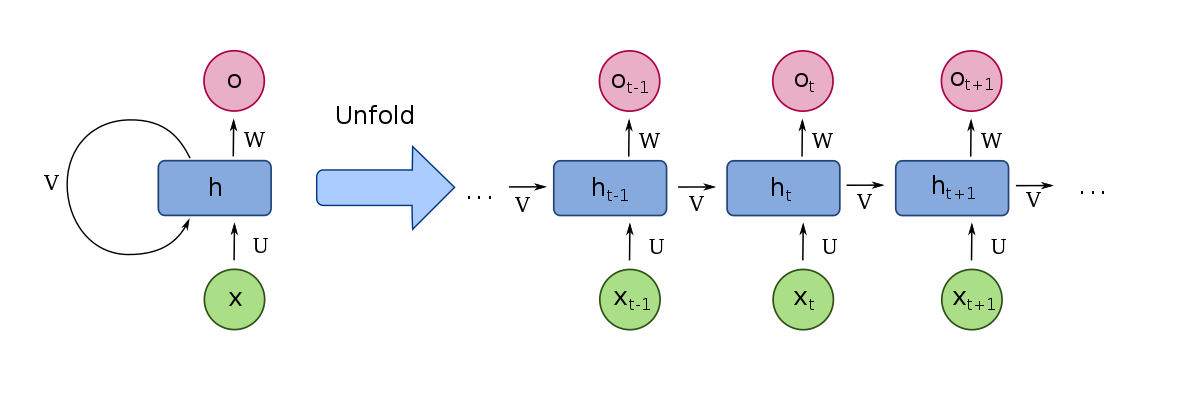
\includegraphics[height=4cm]{pictures/Recurrent_neural_network_unfold.png}
    \caption{Struttura di una RNN}
    \label{fig:RNN}
\end{figure}

Per quanto riguarda la fase di apprendimento dei valori dei pesi, essa si svolge pressappoco come accade nelle reti neurali tradizionali, ossia attraverso la Back Propagation, che nel caso delle RNN viene chiamata Back Propagation Through Time (BPTT). La principale differenza tra le due consiste nella molteplicità dei diversi vettori di pesi che si hanno nel primo caso, i quali vengono tarati scendendo lungo i livelli della rete neurale; nel secondo caso invece sono presenti tre vettori, ma essi vengono modificati basandosi sull'errore commesso negli step temporali in cui gli esempi sono stati presentati alla rete.

Più formalmente, ciò che si fa è calcolare la derivata parziale dell'errore ottenuto sull'output sui pesi $U$, $V$ e $W$. Non è importante come tale errore venga definito, purché ovviamente sia sensato (ad esempio l'MSE per la regressione o l'accuracy per la classificazione). L'errore compiuto dalla RNN è la somma degli errori compiuti nei singoli step.

\begin{equation*}
    \frac{\partial E}{\partial U} = \sum_t{\frac{\partial E_t}{\partial U}}
\end{equation*}

\begin{equation*}
    \frac{\partial E}{\partial V} = \sum_t{\frac{\partial E_t}{\partial V}}
\end{equation*}

\begin{equation*}
    \frac{\partial E}{\partial W} = \sum_t{\frac{\partial E_t}{\partial W}}
\end{equation*}
Si noti che in tutti e tre i casi, essendo $E$ una funzione calcolata sulla base della funzione $o$, si può applicare la regola della catena per le derivate, ottenendo così il seguente risultato (qui viene mostrato solo quello per $W$, ma la situazione è analoga anche per $U$ e $V$)

\begin{equation*}
    \frac{\partial E}{\partial W} = \sum_t{\frac{\partial E_t}{\partial o_t}\frac{\partial o_t}{\partial W}}
\end{equation*}

Si noti anche che per il calcolo di $\frac{\partial o_t}{\partial W}$ è relativamente semplice, perché $W$ influisce direttamente sul valore dell'output, negli altri due casi invece si rende necessario l'uso di tutte le componenti della rete.

\begin{align*}
    \frac{\partial o_t}{\partial V} = \sum_{t'=1}^t{\frac{\partial o_t}{\partial h_t}\frac{\partial h_t}{\partial h_t'}\frac{\partial h_t'}{\partial V}}     &&     dove \ \ \frac{\partial h_t}{\partial h_{t'}} = \prod_{j=t'+1}^t {\frac{\partial h_j}{\partial h_{j-1}}}
\end{align*}
La versione con $U$ è simile a quella riportata sopra.

Dall'ultima equazione si possono osservare due problemi, entrambi legati al livello nascosto. Infatti per il calcolo del gradiente vengono sfruttati tutti i valori $h_t$ generati da $t=0$ fino al $t$ corrente. Non è quindi difficile intuire che per sequenze molto lunghe questo approccio risulti essere computazionalmente oneroso.

Un secondo problema, forse meno intuitivo, è la sensibilità delle RNN al gradient vanishing. A causa della natura delle funzioni di attivazione sfruttate solitamente ($tanh$ o sigmoide), il calcolo della derivata restituisce dei valori compresi tra 0 e 1, nel caso della $tanh$ e tra 0 e 0,25 nel caso della sigmoide (v. \figurename~\ref{fig:sigm_tanh}) e, a causa dei molti prodotti tra le derivate causati dalla regola della catena, i valori che andranno atti ad aggiornare i pesi saranno sempre più piccoli in valore assoluto, fino a rendere praticamente inesistente l'apprendimento una volta superati un certo numero di step temporali.

\begin{figure}
    \centering
    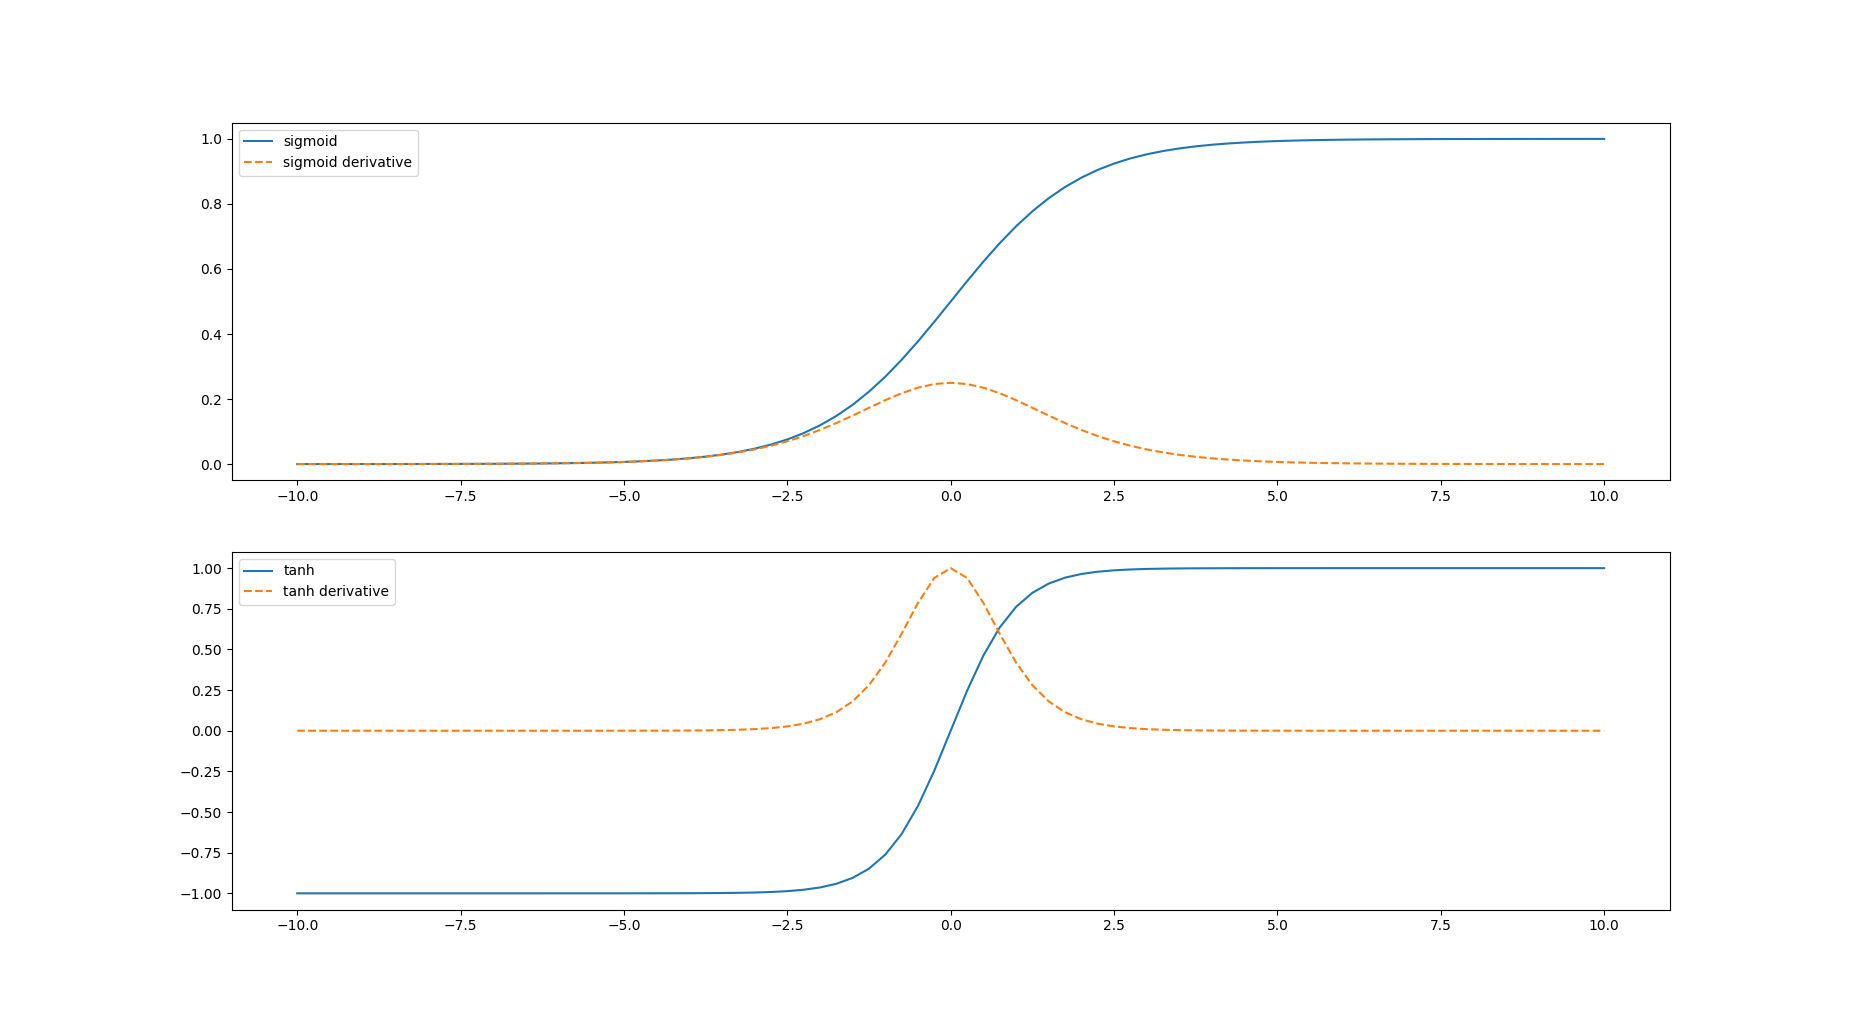
\includegraphics[height=7cm]{pictures/sigm_tanh_deriv.png}
    \caption{Sigmoide, tanh e rispettive derivate}
    \label{fig:sigm_tanh}
\end{figure}

Una soluzione tipica per ovviare al problema del gradient vanishing è quella di usare una diversa funzione di attivazione, generalmente la ReLU o sue varianti.

\begin{equation*}
    ReLU(x) = max(0,x)
\end{equation*}
Essa si caratterizza per essere lineare per valori superiori allo 0.

Ciò che comunque spesso si fa nelle RNN è anche troncare la BPTT a pochi istanti temporali prima di quello attuale, in modo da non rendere troppo lunghi i tempi di computazione e di ridurre l'effetto del gradient vanishing. Purtroppo questa soluzione impedisce alla RNN di cogliere dipendenze tra elementi della sequenza distanti tra loro, il che le rende effettivamente utilizzabili solo in casi semplici.

Allo stato dell'arte viene usata una versione più complessa della RNN esposta finora, detta LSTM. Nel progetto svolto per questa tesi, è stata sfruttata una LSTM.

\subsubsection{LSTM}